%%%%%%%%%%%%%%%%%%%%%%%%%%%%%%%%%%%%%%%%%%%%%%%%%%%%%%%%%%%%%%%%%%%%%%
\begin{frame}[fragile]\frametitle{}
\begin{center}
{\Large Algorithms}
\end{center}

\end{frame}

%%%%%%%%%%%%%%%%%%%%%%%%%%%%%%%%%%%%%%%%%%%%%%%%%%%%%%%%%%%%%%%%%%%%%%
\begin{frame}[fragile]\frametitle{}
\begin{center}
{\Large Sorting}
\end{center}

\end{frame}


\begin{frame}
	\frametitle{BogoSort}
		\begin{block}{BogoSort}
			The easiest form of sorting: Just try all permutations of the list.
		\end{block}	
		\pause
		\begin{block}{Time complexity?}
			\begin{enumerate}[A.]
				\item $\Theta(n)$
				\item $\Theta(n^2)$
				\item $\Theta(2^n)$
				\item $\Theta(n^n)$
				\item $\Theta(n!)$
				\item I don't know
			\end{enumerate}
		\end{block}
	
\end{frame}

\begin{frame}
	\frametitle{Some questions and answers}
\begin{block}{The scope of our problem}
	Some observations and questions.
	\begin{itemize}
		\item The solution space is huge: $n!$ for $n$ items.
			\pause
		\item The use case is not uncommon, so we hope/look for an efficient (polynomial time) algorithm.
			\pause
		\item Humans have a lot of experience sorting items, can we use those strategies?
			\pause
		\item Or are there methods that computers excel at, that would be terrible for humans?
	\end{itemize}
\end{block}	
\pause
\begin{block}{Yes!}
	\begin{itemize}
		\item There are polynomial time algorithms,
			\pause
		\item We can translate our own methods,
		\item But computers can definitely do better.
	\end{itemize}
\end{block}
\end{frame}

\begin{frame}
	\frametitle{Use case?}
	\begin{block}{Why?}
		What do we use sorting for?
	\end{block}
	\pause
	\begin{block}{Many things!}
		\begin{itemize}
			\item Books in the library.
			\item Exams for an exam review.
			\item Closest pair of points.
			\item Convex hulls.
			\item Efficient look-ups in lists that do not change.
			\item And many many more (see also later lectures in graph algorithms).
		\end{itemize}	
	\end{block}
\end{frame}

%%%%%%%%%%%%%%%%%%%%%%%%%%%%%%%%%%%%%%%%%%%%%%%%%%%%%%%%%%%%%%%%%%%%%%
\begin{frame}[fragile]\frametitle{}
\begin{center}
{\Large Bubble Sort}
\end{center}

\end{frame}



\begin{frame}
	\frametitle{Bubble sort}
	\framesubtitle{Getting rid of inversions}
	
	\begin{overlayarea}{\textwidth}{\textheight}
		\only<1>{
			\begin{block}{Let's formalise}
				What did you do yesterday?
			\end{block}
		}
		
			\pause
			\begin{block}{Your algorithm}
				\begin{block}
					While $v_i > v_{i+1}$ for some $i$
						State Switch them around.	
					EndWhile
				\end{block}
			\end{block}
			\pause
			\begin{center}
			\begin{tikzpicture}[scale=0.85, transform shape]
	\only<3>{
		\foreach \x/\val in {0/1,1/20,2/42,3/22,4/17}{
			\node[draw,rectangle, fill=gray!10, minimum size =1cm] (c) at (\x,0) {\val};
		}
	}
	\only<4>{
		\foreach \x/\val/\col in {0/1/green,1/20/green,2/42/black,3/22/black,4/17/black}{
			\node[draw=\col,rectangle, fill=\col!10, minimum size =1cm] (c) at (\x,0) {\val};
		}
	}
	\only<5>{
		\foreach \x/\val/\col in {0/1/black,1/20/green,2/42/green,3/22/black,4/17/black}{
			\node[draw=\col,rectangle, fill=\col!10, minimum size =1cm] (c) at (\x,0) {\val};
		}
	}
	\only<6>{
		\foreach \x/\val/\col in {0/1/black,1/20/black,2/42/red,3/22/red,4/17/black}{
			\node[draw=\col,rectangle, fill=\col!10, minimum size =1cm] (c) at (\x,0) {\val};
		}
	}
	\only<7>{
		\foreach \x/\val/\col in {0/1/black,1/20/black,2/22/green,3/42/green,4/17/black}{
			\node[draw=\col,rectangle, fill=\col!10, minimum size =1cm] (c) at (\x,0) {\val};
		}
	}
	\only<8>{
		\foreach \x/\val/\col in {0/1/black,1/20/black,2/22/black,3/42/red,4/17/red}{
			\node[draw=\col,rectangle, fill=\col!10, minimum size =1cm] (c) at (\x,0) {\val};
		}
	}
	\only<9>{
		\foreach \x/\val/\col in {0/1/black,1/20/black,2/22/black,3/17/green,4/42/green}{
			\node[draw=\col,rectangle, fill=\col!10, minimum size =1cm] (c) at (\x,0) {\val};
		}
	}
	\only<10>{
		\foreach \x/\val/\col in {0/1/green,1/20/green,2/22/black,3/17/black,4/42/black}{
			\node[draw=\col,rectangle, fill=\col!10, minimum size =1cm] (c) at (\x,0) {\val};
		}
	}
	\only<11>{
		\foreach \x/\val/\col in {0/1/black,1/20/green,2/22/green,3/17/black,4/42/black}{
			\node[draw=\col,rectangle, fill=\col!10, minimum size =1cm] (c) at (\x,0) {\val};
		}
	}
	\only<12>{
		\foreach \x/\val/\col in {0/1/black,1/20/black,2/22/red,3/17/red,4/42/black}{
			\node[draw=\col,rectangle, fill=\col!10, minimum size =1cm] (c) at (\x,0) {\val};
		}
	}
	\only<13>{
		\foreach \x/\val/\col in {0/1/black,1/20/black,2/17/green,3/22/green,4/42/black}{
			\node[draw=\col,rectangle, fill=\col!10, minimum size =1cm] (c) at (\x,0) {\val};
		}
	}
	\only<14>{
		\foreach \x/\val/\col in {0/1/black,1/20/black,2/17/black,3/22/green,4/42/green}{
			\node[draw=\col,rectangle, fill=\col!10, minimum size =1cm] (c) at (\x,0) {\val};
		}
	}
	\only<15>{
		\foreach \x/\val/\col in {0/1/green,1/20/green,2/17/black,3/22/black,4/42/black}{
			\node[draw=\col,rectangle, fill=\col!10, minimum size =1cm] (c) at (\x,0) {\val};
		}
	}
	\only<16>{
		\foreach \x/\val/\col in {0/1/black,1/20/red,2/17/red,3/22/black,4/42/black}{
			\node[draw=\col,rectangle, fill=\col!10, minimum size =1cm] (c) at (\x,0) {\val};
		}
	}
	\only<17>{
		\foreach \x/\val/\col in {0/1/black,1/17/green,2/20/green,3/22/black,4/42/black}{
			\node[draw=\col,rectangle, fill=\col!10, minimum size =1cm] (c) at (\x,0) {\val};
		}
	}
	\only<18>{
		\foreach \x/\val/\col in {0/1/black,1/17/black,2/20/green,3/22/green,4/42/black}{
			\node[draw=\col,rectangle, fill=\col!10, minimum size =1cm] (c) at (\x,0) {\val};
		}
	}
	\only<19>{
		\foreach \x/\val/\col in {0/1/black,1/17/black,2/20/black,3/22/green,4/42/green}{
			\node[draw=\col,rectangle, fill=\col!10, minimum size =1cm] (c) at (\x,0) {\val};
		}
	}
	\only<20>{
		\foreach \x/\val/\col in {0/1/green,1/17/green,2/20/black,3/22/black,4/42/black}{
			\node[draw=\col,rectangle, fill=\col!10, minimum size =1cm] (c) at (\x,0) {\val};
		}
	}
	\only<21>{
		\foreach \x/\val/\col in {0/1/black,1/17/green,2/20/green,3/22/black,4/42/black}{
			\node[draw=\col,rectangle, fill=\col!10, minimum size =1cm] (c) at (\x,0) {\val};
		}
	}
	\only<22>{
		\foreach \x/\val/\col in {0/1/black,1/17/black,2/20/green,3/22/green,4/42/black}{
			\node[draw=\col,rectangle, fill=\col!10, minimum size =1cm] (c) at (\x,0) {\val};
		}
	}
	\only<23->{
		\foreach \x/\val/\col in {0/1/black,1/17/black,2/20/black,3/22/green,4/42/green}{
			\node[draw=\col,rectangle, fill=\col!10, minimum size =1cm] (c) at (\x,0) {\val};
		}
	}
\end{tikzpicture}

			\end{center}
			\only<24->{
			\begin{block}{Sounds easy...}
				So how many inversions can there be?
				% \begin{multicols}{2}
				\begin{enumerate}[A.]
					\item $\Theta(n)$
					\item $\Theta(n^2)$
					\item $\Theta(n^n)$
					\item $\Theta(n!)$
				\end{enumerate}
			% \end{multicols}
			\end{block}
		}
	\end{overlayarea}
\end{frame}

\begin{frame}
	\frametitle{The number of inversions}
	\framesubtitle{What is the worst-case?}

	\begin{block}{A list in reverse order}
		Remember yesterday? The people that were at the wrong end took the longest!\\
		\pause
		Consider a list in reverse order:
		\begin{itemize}
			\item The first element is wrong compared to all others: $n-1$ inversions.
		\pause
			\item The second is also wrong with all the ones that come after it: $n-2$ extra inversions.
			\item ...
		\pause
			\item The one-but last one is also wrong with the last one: $1$ inversion
		\pause
			\item So $\Theta(n^2)$ inversion!
		\end{itemize}
	\end{block}
\end{frame}

\begin{frame}
	\frametitle{To summarise in code}
	\begin{columns}
		\column{0.565\textwidth}
	\lstinputlisting{src/bs.py}
		\column{0.455\textwidth}
		\begin{block}{Pros and Cons?}
			What are the pros and cons of bubblesort? Hint: remember I told you it was slow!
		\end{block}
	\end{columns}
\end{frame}

\begin{frame}
	\frametitle{Bubblesort: Pros and Cons}

		\begin{block}{Bubblesort}
			While there are inversions: fix them.
		\end{block}	
		\begin{block}{Pros}
			\begin{itemize}
				\item Great in a distributed setting, with autonomous agents (like students in a lecture hall).
				\item When implemented as: ``continue while there are inversion'' can terminate after one iteration over a
					sorted list! 
				\item Easiest to implement.
			\end{itemize}
		\end{block}	
		\begin{block}{Cons}
			\begin{itemize}
				\item Terribly slow! (Often still slower than other $\Theta(n^2)$ algorithms we will see later)
			\end{itemize}
		\end{block}	
\end{frame}

%%%%%%%%%%%%%%%%%%%%%%%%%%%%%%%%%%%%%%%%%%%%%%%%%%%%%%%%%%%%%%%%%%%%%%
\begin{frame}[fragile]\frametitle{}
\begin{center}
{\Large Bucket Sort}
\end{center}

\end{frame}

\begin{frame}
	\frametitle{Bucket Sort}
	\framesubtitle{The Stephen Tatlock algorithm\dots \only<3->{\tiny Okay that was probably too obscure a reference}}

		\begin{block}{Bucket Sort}
			\begin{enumerate}
				\item Sort the items into buckets (e.g. based on first letter of last name).
					\pause
				\item Sort every bucket.
					\pause
				\item Concatenate all buckets together.
			\end{enumerate}
		\end{block}	
		\pause
		\vspace{-0.2cm}
		\begin{block}{Why is this good?}
			Why should we use this?
		\end{block}
		\pause
		\vspace{-0.2cm}
		\begin{block}{Well...}
			\begin{itemize}
				\item Great for parallelisation!
				\item Great for humans (sorting a bucket can be done using a different algorithm, everyone can pick their own
					favourite).
				\item Average case analysis is interesting for this algorithm (and gets us to something close to linear time for
					average case).
			\end{itemize}
		\end{block}
\end{frame}

%%%%%%%%%%%%%%%%%%%%%%%%%%%%%%%%%%%%%%%%%%%%%%%%%%%%%%%%%%%%%%%%%%%%%%
\begin{frame}[fragile]\frametitle{}
\begin{center}
{\Large Selection Sort}
\end{center}

\end{frame}

\begin{frame}
	\frametitle{Selection Sort}
		\begin{block}{The smallest of variations...}
			Rather than shifting every element to it's correct place\dots\\
			\pause
			We instead repeatedly search for the smallest element and put it at the end of our sorted list/sorted part.
		\end{block}	
	\begin{center}
	\section{Selection Sort}
\label{sec:selection_sort}

\begin{frame}
	\frametitle{Selection Sort}
		\begin{block}{The smallest of variations...}
			Rather than shifting every element to it's correct place\dots\\
			\pause
			We instead repeatedly search for the smallest element and put it at the end of our sorted list/sorted part.
		\end{block}	
	\begin{center}
	\section{Selection Sort}
\label{sec:selection_sort}

\begin{frame}
	\frametitle{Selection Sort}
		\begin{block}{The smallest of variations...}
			Rather than shifting every element to it's correct place\dots\\
			\pause
			We instead repeatedly search for the smallest element and put it at the end of our sorted list/sorted part.
		\end{block}	
	\begin{center}
	\section{Selection Sort}
\label{sec:selection_sort}

\begin{frame}
	\frametitle{Selection Sort}
		\begin{block}{The smallest of variations...}
			Rather than shifting every element to it's correct place\dots\\
			\pause
			We instead repeatedly search for the smallest element and put it at the end of our sorted list/sorted part.
		\end{block}	
	\begin{center}
	\input{figures/tikz/selectionsort.tex}
	\end{center}
\end{frame}

\begin{frame}
	\frametitle{Implementation}
	\begin{exampleblock}{Time Complexity}
		Still $\Theta(n^2)$ as we need to find the minimum $O(n)$ times, which takes $O(n)$ time.
		\end{exampleblock}	
	\begin{alertblock}{See next week's homework}
		You will tell me next week ;)
	\end{alertblock}	
\end{frame}

\begin{frame}
	\frametitle{In-place sorting algorithms}
	\framesubtitle{I'm not going anywhere!}

	\begin{itemize}
		\item The sorting algorithms we have seen so-far are \alert{in-place} sorting algorithms.
			\pause
		\item They take a list and modify that list to become sorted.
			\pause
		\item Of course we can also make them not in-place, by first making a copy of the list and sorting that.
			\pause
		\item But after the break (when we discuss merge sort) we will see an example of an algorithm that is easier to make
			not in-place.
	\end{itemize}
\end{frame}



	\end{center}
\end{frame}

\begin{frame}
	\frametitle{Implementation}
	\begin{exampleblock}{Time Complexity}
		Still $\Theta(n^2)$ as we need to find the minimum $O(n)$ times, which takes $O(n)$ time.
		\end{exampleblock}	
	\begin{alertblock}{See next week's homework}
		You will tell me next week ;)
	\end{alertblock}	
\end{frame}

\begin{frame}
	\frametitle{In-place sorting algorithms}
	\framesubtitle{I'm not going anywhere!}

	\begin{itemize}
		\item The sorting algorithms we have seen so-far are \alert{in-place} sorting algorithms.
			\pause
		\item They take a list and modify that list to become sorted.
			\pause
		\item Of course we can also make them not in-place, by first making a copy of the list and sorting that.
			\pause
		\item But after the break (when we discuss merge sort) we will see an example of an algorithm that is easier to make
			not in-place.
	\end{itemize}
\end{frame}



	\end{center}
\end{frame}

\begin{frame}
	\frametitle{Implementation}
	\begin{exampleblock}{Time Complexity}
		Still $\Theta(n^2)$ as we need to find the minimum $O(n)$ times, which takes $O(n)$ time.
		\end{exampleblock}	
	\begin{alertblock}{See next week's homework}
		You will tell me next week ;)
	\end{alertblock}	
\end{frame}

\begin{frame}
	\frametitle{In-place sorting algorithms}
	\framesubtitle{I'm not going anywhere!}

	\begin{itemize}
		\item The sorting algorithms we have seen so-far are \alert{in-place} sorting algorithms.
			\pause
		\item They take a list and modify that list to become sorted.
			\pause
		\item Of course we can also make them not in-place, by first making a copy of the list and sorting that.
			\pause
		\item But after the break (when we discuss merge sort) we will see an example of an algorithm that is easier to make
			not in-place.
	\end{itemize}
\end{frame}



	\end{center}
\end{frame}

\begin{frame}
	\frametitle{Implementation}
	\begin{block}{Time Complexity}
		Still $\Theta(n^2)$ as we need to find the minimum $O(n)$ times, which takes $O(n)$ time.
		\end{block}	
	\begin{block}{See next week's homework}
		You will tell me next week ;)
	\end{block}	
\end{frame}

\begin{frame}
	\frametitle{In-place sorting algorithms}
	\framesubtitle{I'm not going anywhere!}

	\begin{itemize}
		\item The sorting algorithms we have seen so-far are \alert{in-place} sorting algorithms.
			\pause
		\item They take a list and modify that list to become sorted.
			\pause
		\item Of course we can also make them not in-place, by first making a copy of the list and sorting that.
			\pause
		\item But after the break (when we discuss merge sort) we will see an example of an algorithm that is easier to make
			not in-place.
	\end{itemize}
\end{frame}

%%%%%%%%%%%%%%%%%%%%%%%%%%%%%%%%%%%%%%%%%%%%%%%%%%%%%%%%%%%%%%%%%%%%%%
\begin{frame}[fragile]\frametitle{}
\begin{center}
{\Large Insertion Sort}
\end{center}

\end{frame}

\begin{frame}
	\frametitle{Insertion Sort}
	\framesubtitle{How does that work?}
		\begin{block}{Insertion Sort}
			The main idea:
			\begin{itemize}
				\item We build the list, step by step.
					\pause
				\item We keep our intermediate result sorted.
					\pause
				\item At every step, we insert the next element into the right place.
					\pause
				\item This means we need to shift over (worst-case) $n$ elements for every element we insert...
					\pause
				\item So in total $\Theta(n^2)$ time.
			\end{itemize}
		\end{block}
\end{frame}

\begin{frame}
	\frametitle{Insertion Sort}
	\begin{block}
		State $i gets 1$ Comment {The first element forms a sorted list on it's own}
		\pause
		While $i < \texttt{len}(l)$
		State $j gets i$
		\pause
		While $j > 0$ and $v_{j-1} < v_{j}$ 
			State swap $v_j$ and $v_{j-1}$	
			State $j gets j -1$
		EndWhile
		\pause
		State $i gets i+1$
		EndWhile
	\end{block}
	\pause
	\begin{center}
	\section{Insertion Sort}
\label{sec:insertion_sort}

\begin{frame}
	\frametitle{Insertion sort}
	\begin{center}
		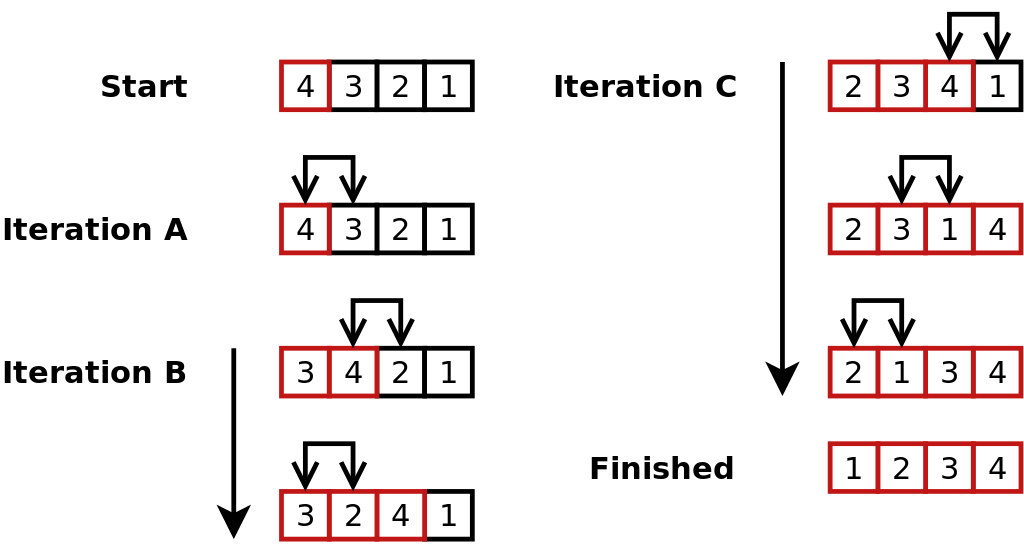
\includegraphics[width=0.8\textwidth]{figures/insertionsort.png}\\
		\hspace*{15pt}\hbox{\scriptsize Image By:\thinspace{\itshape MrDrBob}}
		% https://commons.wikimedia.org/wiki/File:Insertion-sort.svg
	\end{center}
\end{frame}

\begin{frame}
	\frametitle{Insertion Sort}
	\framesubtitle{How does that work?}
		\begin{block}{Insertion Sort}
			The main idea:
			\begin{itemize}
				\item We build the list, step by step.
					\pause
				\item We keep our intermediate result sorted.
					\pause
				\item At every step, we insert the next element into the right place.
					\pause
				\item This means we need to shift over (worst-case) $n$ elements for every element we insert...
					\pause
				\item So in total $\Theta(n^2)$ time.
			\end{itemize}
		\end{block}
\end{frame}

\begin{frame}
	\frametitle{Insertion Sort}
	\begin{algorithmic}
		\State $i \gets 1$ \Comment{The first element forms a sorted list on it's own}
		\pause
		\While{$i < \texttt{len}(l)$}
		\State $j \gets i$
		\pause
		\While{$j > 0$ and $v_{j-1} < v_{j}$}
			\State swap $v_j$ and $v_{j-1}$	
			\State $j \gets j -1$
		\EndWhile
		\pause
		\State $i \gets i+1$
		\EndWhile
	\end{algorithmic}
	\pause
	\begin{center}
	\section{Insertion Sort}
\label{sec:insertion_sort}

\begin{frame}
	\frametitle{Insertion sort}
	\begin{center}
		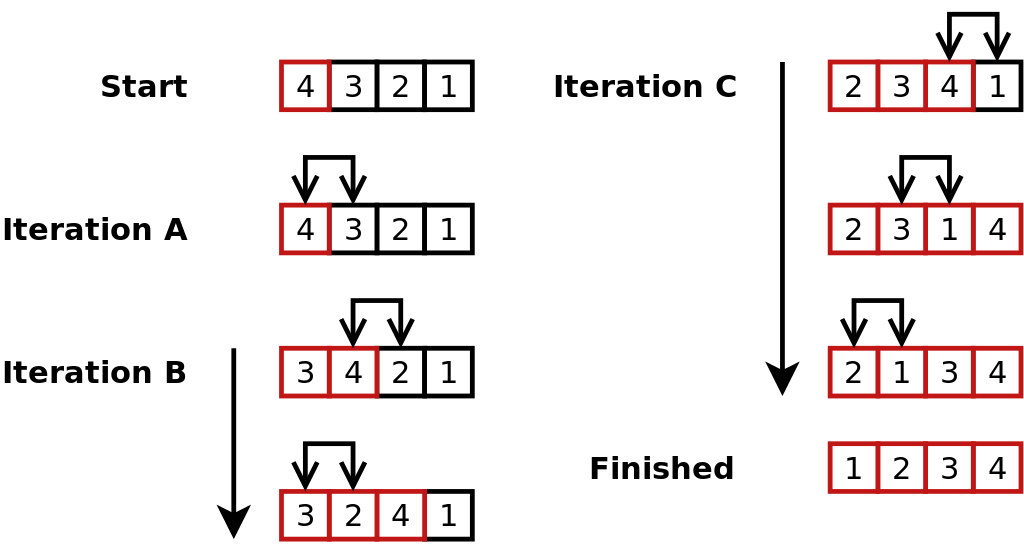
\includegraphics[width=0.8\textwidth]{figures/insertionsort.png}\\
		\hspace*{15pt}\hbox{\scriptsize Image By:\thinspace{\itshape MrDrBob}}
		% https://commons.wikimedia.org/wiki/File:Insertion-sort.svg
	\end{center}
\end{frame}

\begin{frame}
	\frametitle{Insertion Sort}
	\framesubtitle{How does that work?}
		\begin{block}{Insertion Sort}
			The main idea:
			\begin{itemize}
				\item We build the list, step by step.
					\pause
				\item We keep our intermediate result sorted.
					\pause
				\item At every step, we insert the next element into the right place.
					\pause
				\item This means we need to shift over (worst-case) $n$ elements for every element we insert...
					\pause
				\item So in total $\Theta(n^2)$ time.
			\end{itemize}
		\end{block}
\end{frame}

\begin{frame}
	\frametitle{Insertion Sort}
	\begin{algorithmic}
		\State $i \gets 1$ \Comment{The first element forms a sorted list on it's own}
		\pause
		\While{$i < \texttt{len}(l)$}
		\State $j \gets i$
		\pause
		\While{$j > 0$ and $v_{j-1} < v_{j}$}
			\State swap $v_j$ and $v_{j-1}$	
			\State $j \gets j -1$
		\EndWhile
		\pause
		\State $i \gets i+1$
		\EndWhile
	\end{algorithmic}
	\pause
	\begin{center}
	\section{Insertion Sort}
\label{sec:insertion_sort}

\begin{frame}
	\frametitle{Insertion sort}
	\begin{center}
		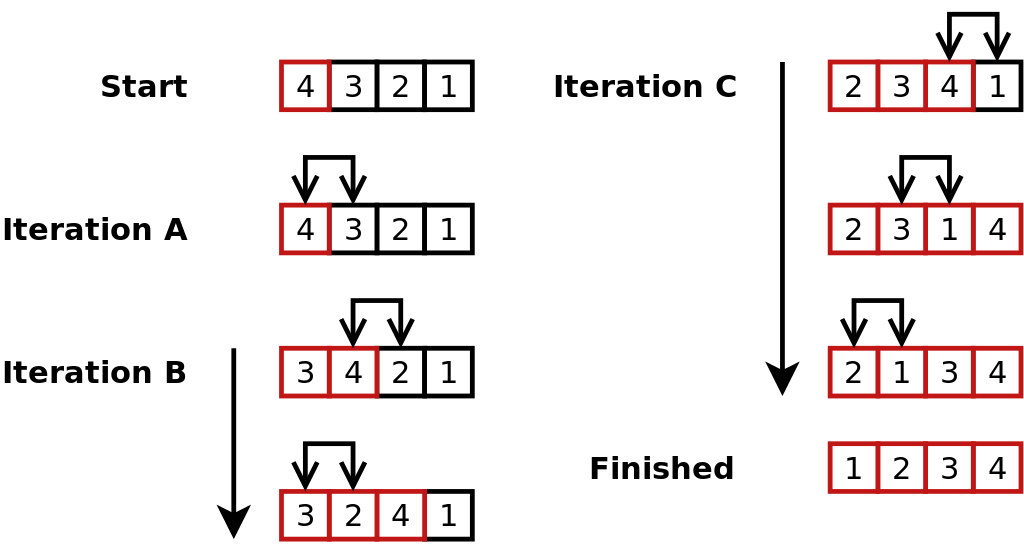
\includegraphics[width=0.8\textwidth]{figures/insertionsort.png}\\
		\hspace*{15pt}\hbox{\scriptsize Image By:\thinspace{\itshape MrDrBob}}
		% https://commons.wikimedia.org/wiki/File:Insertion-sort.svg
	\end{center}
\end{frame}

\begin{frame}
	\frametitle{Insertion Sort}
	\framesubtitle{How does that work?}
		\begin{block}{Insertion Sort}
			The main idea:
			\begin{itemize}
				\item We build the list, step by step.
					\pause
				\item We keep our intermediate result sorted.
					\pause
				\item At every step, we insert the next element into the right place.
					\pause
				\item This means we need to shift over (worst-case) $n$ elements for every element we insert...
					\pause
				\item So in total $\Theta(n^2)$ time.
			\end{itemize}
		\end{block}
\end{frame}

\begin{frame}
	\frametitle{Insertion Sort}
	\begin{algorithmic}
		\State $i \gets 1$ \Comment{The first element forms a sorted list on it's own}
		\pause
		\While{$i < \texttt{len}(l)$}
		\State $j \gets i$
		\pause
		\While{$j > 0$ and $v_{j-1} < v_{j}$}
			\State swap $v_j$ and $v_{j-1}$	
			\State $j \gets j -1$
		\EndWhile
		\pause
		\State $i \gets i+1$
		\EndWhile
	\end{algorithmic}
	\pause
	\begin{center}
	\input{figures/tikz/insertionsort.tex}
	\end{center}
\end{frame}

\begin{frame}
	\frametitle{Would you like some sausages with your cheese?}
	\begin{columns}
		\column{0.455\textwidth}
		\begin{algorithmic}
			\State $i \gets 1$ 
			\While{$i < \texttt{len}(l)$}
			\State $j \gets i$
			\While{$j > 0$ and $v_j < v_{j-1}$}
			\State swap $v_j$ and $v_{j-1}$	
			\State $j \gets j -1$
			\EndWhile
			\State $i \gets i+1$
			\EndWhile
		\end{algorithmic}
		\column{0.455\textwidth}
		\begin{questionblock}{Run time}
			What instance of a list would give the worst performance here?	
		\end{questionblock}
		\pause
		\begin{answerblock}{Again!?}
			Once again it is the reverse list, where every item needs to be moved to the front requiring most swaps.
		\end{answerblock}
		\pause
			\begin{block}{So...}
				The run time is still $\Theta(n^2)$.
			\end{block}	
	\end{columns}

	
\end{frame}

\begin{frame}
	\frametitle{Implementation to summarise}
	
		\begin{alertblock}{See you tomorrow!}
			We will implement this tomorrow :)
		\end{alertblock}	
\end{frame}

\begin{frame}
	\frametitle{Insertion Sort: Pros and Cons}
		\begin{block}{Insertion Sort}
			Repeatedly insert the next item in the correct place in a sorted list.
		\end{block}	
		\begin{exampleblock}{Pros}
			\begin{itemize}
				\item `Easy' algorithm to implement.
				\item Good performance for an $O(n^2)$ algorithm.
			\end{itemize}
		\end{exampleblock}	
		\begin{alertblock}{Cons}
			\begin{itemize}
				\item Still not as fast as comparison-based sorting algorithms can be.
			\end{itemize}
		\end{alertblock}	
	
\end{frame}

	\end{center}
\end{frame}

\begin{frame}
	\frametitle{Would you like some sausages with your cheese?}
	\begin{columns}
		\column{0.455\textwidth}
		\begin{algorithmic}
			\State $i \gets 1$ 
			\While{$i < \texttt{len}(l)$}
			\State $j \gets i$
			\While{$j > 0$ and $v_j < v_{j-1}$}
			\State swap $v_j$ and $v_{j-1}$	
			\State $j \gets j -1$
			\EndWhile
			\State $i \gets i+1$
			\EndWhile
		\end{algorithmic}
		\column{0.455\textwidth}
		\begin{questionblock}{Run time}
			What instance of a list would give the worst performance here?	
		\end{questionblock}
		\pause
		\begin{answerblock}{Again!?}
			Once again it is the reverse list, where every item needs to be moved to the front requiring most swaps.
		\end{answerblock}
		\pause
			\begin{block}{So...}
				The run time is still $\Theta(n^2)$.
			\end{block}	
	\end{columns}

	
\end{frame}

\begin{frame}
	\frametitle{Implementation to summarise}
	
		\begin{alertblock}{See you tomorrow!}
			We will implement this tomorrow :)
		\end{alertblock}	
\end{frame}

\begin{frame}
	\frametitle{Insertion Sort: Pros and Cons}
		\begin{block}{Insertion Sort}
			Repeatedly insert the next item in the correct place in a sorted list.
		\end{block}	
		\begin{exampleblock}{Pros}
			\begin{itemize}
				\item `Easy' algorithm to implement.
				\item Good performance for an $O(n^2)$ algorithm.
			\end{itemize}
		\end{exampleblock}	
		\begin{alertblock}{Cons}
			\begin{itemize}
				\item Still not as fast as comparison-based sorting algorithms can be.
			\end{itemize}
		\end{alertblock}	
	
\end{frame}

	\end{center}
\end{frame}

\begin{frame}
	\frametitle{Would you like some sausages with your cheese?}
	\begin{columns}
		\column{0.455\textwidth}
		\begin{algorithmic}
			\State $i \gets 1$ 
			\While{$i < \texttt{len}(l)$}
			\State $j \gets i$
			\While{$j > 0$ and $v_j < v_{j-1}$}
			\State swap $v_j$ and $v_{j-1}$	
			\State $j \gets j -1$
			\EndWhile
			\State $i \gets i+1$
			\EndWhile
		\end{algorithmic}
		\column{0.455\textwidth}
		\begin{questionblock}{Run time}
			What instance of a list would give the worst performance here?	
		\end{questionblock}
		\pause
		\begin{answerblock}{Again!?}
			Once again it is the reverse list, where every item needs to be moved to the front requiring most swaps.
		\end{answerblock}
		\pause
			\begin{block}{So...}
				The run time is still $\Theta(n^2)$.
			\end{block}	
	\end{columns}

	
\end{frame}

\begin{frame}
	\frametitle{Implementation to summarise}
	
		\begin{alertblock}{See you tomorrow!}
			We will implement this tomorrow :)
		\end{alertblock}	
\end{frame}

\begin{frame}
	\frametitle{Insertion Sort: Pros and Cons}
		\begin{block}{Insertion Sort}
			Repeatedly insert the next item in the correct place in a sorted list.
		\end{block}	
		\begin{exampleblock}{Pros}
			\begin{itemize}
				\item `Easy' algorithm to implement.
				\item Good performance for an $O(n^2)$ algorithm.
			\end{itemize}
		\end{exampleblock}	
		\begin{alertblock}{Cons}
			\begin{itemize}
				\item Still not as fast as comparison-based sorting algorithms can be.
			\end{itemize}
		\end{alertblock}	
	
\end{frame}

	\end{center}
\end{frame}

\begin{frame}
	\frametitle{Would you like some sausages with your cheese?}
	\begin{columns}
		\column{0.455\textwidth}
		\begin{block}
			State $i \gets 1$ 
			While $i < \texttt{len}(l)$
			State $j \gets i$
			While $j > 0$ and $v_j < v_{j-1}$
			State swap $v_j$ and $v_{j-1}$	
			State $j \gets j -1$
			EndWhile
			State $i \gets i+1$
			EndWhile
		\end{block}
		\column{0.455\textwidth}
		\begin{block}{Run time}
			What instance of a list would give the worst performance here?	
		\end{block}
		\pause
		\begin{block}{Again!?}
			Once again it is the reverse list, where every item needs to be moved to the front requiring most swaps.
		\end{block}
		\pause
			\begin{block}{So...}
				The run time is still $\Theta(n^2)$.
			\end{block}	
	\end{columns}

	
\end{frame}

\begin{frame}
	\frametitle{Implementation to summarise}
	
		\begin{block}{See you tomorrow!}
			We will implement this tomorrow :)
		\end{block}	
\end{frame}

\begin{frame}
	\frametitle{Insertion Sort: Pros and Cons}
		\begin{block}{Insertion Sort}
			Repeatedly insert the next item in the correct place in a sorted list.
		\end{block}	
		\begin{block}{Pros}
			\begin{itemize}
				\item `Easy' algorithm to implement.
				\item Good performance for an $O(n^2)$ algorithm.
			\end{itemize}
		\end{block}	
		\begin{block}{Cons}
			\begin{itemize}
				\item Still not as fast as comparison-based sorting algorithms can be.
			\end{itemize}
		\end{block}	
	
\end{frame}

%%%%%%%%%%%%%%%%%%%%%%%%%%%%%%%%%%%%%%%%%%%%%%%%%%%%%%%%%%%%%%%%%%%%%%
\begin{frame}[fragile]\frametitle{}
\begin{center}
{\Large Merge Sort}
\end{center}

\end{frame}

\begin{frame}
	\frametitle{Merge Sort}
	\framesubtitle{XKCD Ineffective Sorts: \url{https://xkcd.com/1185/}}
	\begin{center}
		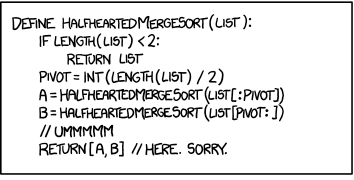
\includegraphics[width=0.8\textwidth]{images/mergesort.png}\\
	\end{center}
\end{frame}

\begin{frame}
	\frametitle{Merge Sort}
	\begin{block}{Merge Sort}
		A recursive sorting algorithm.\\
		\pause
		It splits the list into two, sorts each half, then combines the results.
	\end{block}	
	\pause
	\begin{block}{Not great for humans}
		As you discovered yesterday, this algorithm is not the easiest for humans to perform.
	\end{block}	
	\pause
	\begin{block}{Great for computers}
		But computers do excellent at it!
	\end{block}	
\end{frame}

\begin{frame}
	\frametitle{The idea}
	\begin{overlayarea}{\textwidth}{\textheight}
		\begin{columns}
			\column{0.705\textwidth}
			The algorithm:
		\begin{block}
			\scriptsize
			Function{MergeSort}{xs}
			If{len(xs) $< 2$}	
			State Return xs
			EndIf
			\pause
			State leftHalf $gets$ Call{MergeSort}{the first half of the list}
			State rightHalf $gets$ Call{MergeSort}{the second half of the list}
			\pause
			State result $gets []$, $i gets 0$, $j gets 0$
			While{$i < $ len(leftHalf) and $j < $ len(rightHalf)}
			\only<3>{
				\dots
			}
			\only<4>{
			State\alert{Something goes here}
			State\alert{Update $i$ and $j$ accordingly.}
		}
		\only<5->{
			If{leftHalf[i] $<$ rightHalf[j]}
			State result.append(leftHalf[i]),  $i gets i + 1$
			Else
		}
		\only<5>{
			State 
		}
		\only<6->{
			State result.append(rightHalf[j]),  $j gets j + 1$
		}
		\only<5->{
			EndIf
		}
			EndWhile
			\only<7>{
				State \alert{Something here?}
			}
			\only<8->{
				\tiny
			While{$i < $ len(leftHalf)}
			State result.append(leftHalf[i]),  $i\gets i + 1$
			EndWhile
			While{$j < $ len(rightHalf)}
			State result.append(rightHalf[j]),  $j\gets j + 1$
			EndWhile
		}
		\scriptsize
		State Return result
			EndFunction
		\end{block}
		
			\column{0.305\textwidth}
			\only<4>{
			\begin{block}{What do we do here?}
				\begin{enumerate}[A.]
					\item Compare leftHalf[0] with rightHalf[0]
					\item Compare leftHalf[i] with rightHalf[0]
					\item Compare leftHalf[0] with rightHalf[j]
					\item Compare leftHalf[i] with rightHalf[j]
				\end{enumerate}
			\end{block}
				}
			\only<7>{
			\begin{block}{What do we do here?}
				\begin{enumerate}[A.]
					\item Nothing, we're done
					\item Empty the remainder of the left half, then the right half.
					\item Empty the remainder of the right half, then the left half.
					\item Only one half can still have items left, empty that one.
				\end{enumerate}
			\end{block}
				}
			\only<9->{
				\begin{block}{You can see one con}
					The algorithm is a bit more involved...
			\end{block}
				}
			\only<10->{
				\begin{block}{Is it better?}
					What is a tight bound on the run time?\\
					Hint: you can use the master theorem!
			\end{block}
				}
		\end{columns}
	\end{overlayarea}
\end{frame}

\begin{frame}
	\frametitle{Merge sort run time}
	\begin{block}{Run time}
		$T(0) = T(1) = c_0$ and $T(n) = 2T(n/2) + \Theta(n)$.\\
		This gives $n^{\log_2(2)} = n$ leaves, and as $f(n) = \Theta(n)$ this makes this case 2 of the master method.\\
		Thus $\Theta(n\log n)$ work! We improved!
	\end{block}

	\pause
	\begin{block}{Worst-case instance?}
		What would be the worst type of list for this algorithm?
	\end{block}
	\pause
	\begin{block}{There is none}
		There is no worst-case instance, all of them take $\Theta(n \log n)$ time as we append $n$ items in $\log n$
		recursive calls in the recursion tree.
	\end{block}
\end{frame}

\begin{frame}
	\frametitle{Let's do one example!}
	\begin{block}{But on the smartboard}
		Making this in Tikz is way too much effort ;)
	\end{block}		
\end{frame}

\begin{frame}
	\frametitle{Merge sort: pros and cons}
	\begin{block}{Merge sort}
			Recursively split the list, sort and merge sorted lists.
		\end{block}	
		\begin{block}{Pros}
			\begin{itemize}
				\item Great in a distributed setting, as it can be parallelised!
				\item Great time complexity! $O(n\log n)$
			\end{itemize}
		\end{block}	
		\begin{block}{Cons}
			\begin{itemize}
				\item A bit harder to implement.
				\item Always takes $O(n \log n)$ even when only two items would have to be switched.
			\end{itemize}
		\end{block}	
\end{frame}

%%%%%%%%%%%%%%%%%%%%%%%%%%%%%%%%%%%%%%%%%%%%%%%%%%%%%%%%%%%%%%%%%%%%%%
\begin{frame}[fragile]\frametitle{}
\begin{center}
{\Large Quick Sort}
\end{center}

\end{frame}


\begin{frame}
	\frametitle{Quicksort}
	\framesubtitle{XKCD Ineffective Sorts: \url{https://xkcd.com/1185/}}
	\begin{center}
		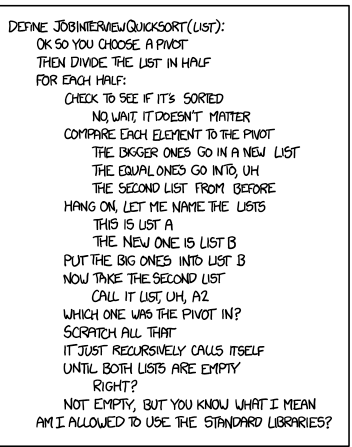
\includegraphics[width=0.4\textwidth]{images/quicksort.png}\\
	\end{center}
\end{frame}

\begin{frame}
	\frametitle{Quicksort}
	\begin{block}{Quicksort}
		A recursive sorting algorithm.\\
		\pause
		It splits the list into two, sorts each half, then combines the results.
	\end{block}	
	\pause
	\begin{block}{Wait...}
		That sounds exactly like mergesort!?
	\end{block}	
	\pause
	\begin{block}{Yes}
		But this is often even better :)
	\end{block}	
\end{frame}

\begin{frame}
	\frametitle{The idea}
	\begin{overlayarea}{\textwidth}{\textheight}
		\begin{columns}
			\column{0.705\textwidth}
			The algorithm:
		\begin{block}
			Function{Quicksort}{xs}
			If{len(xs) $< 2$}	
			State Return xs
			EndIf
			\pause
			State pivot $gets$ some element from xs
			State left $gets$ everything smaller than pivot
			State right $gets$ everything larger than pivot
			State leftHalf $gets$ Call{Quicksort}{left}
			State rightHalf $gets$ Call{Quicksort}{right}
			\pause
			State Return \alt<5->{leftHalf + pivot + rightHalf}{\dots}
			EndFunction
		\end{block}
		
			\column{0.305\textwidth}
			\only<4>{
			\begin{block}{What do we do here?}
				\begin{enumerate}[A.]
					\item Merge the left and right half.
					\item Return left + right
					\item Return left + pivot + right
					\item Return right + pivot + left
				\end{enumerate}
			\end{block}
				}
			\only<6>{
				\begin{block}{What I thought this was better?}
					What is the time complexity of this?\\
					Or rather, what does the worst case input look like?
			\end{block}
				}
		\end{columns}
	\end{overlayarea}
\end{frame}

\begin{frame}
	\frametitle{It depends!}

	\begin{block}{It depends!}
		Everything stands and falls by the choice of pivot.
	\end{block}
	\pause
	\begin{block}{The first element}
		What is the worst input if we always take the first element as the pivot?
		\begin{enumerate}[A.]
			\item A sorted list
			\item The reverse of a sorted list
			\item A list that has the first $n/2$ elements sorted ascendingly and the second $n/2$ elements sorted descendingly.
		\end{enumerate}
	\end{block}
	\pause
	\begin{block}{A sorted list}
	 This takes of only $1$ element every time, meaning we need $O(n^2)$ time.	
	\end{block}
\end{frame}

\begin{frame}
	\frametitle{In practice}
	
		\begin{block}{Quick Sort in the real world}
			\begin{itemize}
				\item It is the most common sorting algorithm used.
				\item The implementations choose \textit{random} pivots.
					\pause
				\item Worst-case this is still $O(n^2)$ of course.
					\pause
				\item But with some fancy analysis (that we will not go into today, but maybe tomorrow ;)), we can show that
					this is $O(n \log n)$ in expectation (average case if you will).
					\pause
				\item In practice this often outperforms merge sort significantly, especially when we make it in-place.
			\end{itemize}
		\end{block}	
\end{frame}

\begin{frame}
	\frametitle{Let's do one example!}
	\begin{block}{But on the smartboard}
		Making this in Tikz is way too much effort ;)
	\end{block}		
\end{frame}

\begin{frame}
	\frametitle{Quicksort: pros and cons}
	\begin{block}{Quicksort}
			Recursively split the list in smaller and larger elements, sort and combine.
		\end{block}	
		\begin{block}{Pros}
			\begin{itemize}
				\item Great time complexity for average case $O(n\log n)$
				\item Simpler to implement (and faster in most cases) than merge sort.
				\item Argument based on authority: the whole world uses it.
			\end{itemize}
		\end{block}	
		\begin{block}{Cons}
			\begin{itemize}
				\item Still $O(n^2)$ if we are unlucky in choosing pivots.
			\end{itemize}
		\end{block}	
\end{frame}

%%%%%%%%%%%%%%%%%%%%%%%%%%%%%%%%%%%%%%%%%%%%%%%%%%%%%%%%%%%%%%%%%%%%%%
\begin{frame}[fragile]\frametitle{}
\begin{center}
{\Large Sorting Summary}
\end{center}

\end{frame}

\begin{frame}
	\frametitle{To summarise}
	\framesubtitle{XKCD Ineffective Sorts: \url{https://xkcd.com/1185/}}
	\begin{center}
		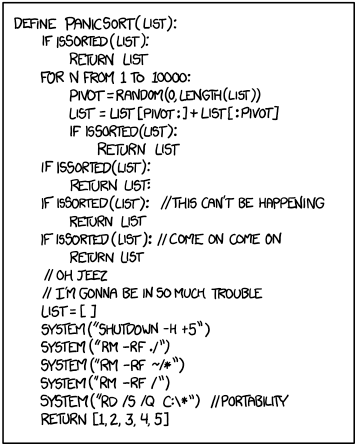
\includegraphics[width=0.4\textwidth]{images/panicsort.png}\\
	\end{center}
\end{frame}
	
\begin{frame}
	\frametitle{Summary table}
	\begin{tabular}{r | c | c | c}
		\small
		Sorting method & Time & Main advantage & Main disadvantage \\
		\midrule
		Bubble Sort & $O(n^2)$ & Easy for humans! &  Very very very very slow \\
		Insertion Sort & $O(n^2)$ & Good for small lists &  Still quadratic time \\
		Selection Sort & $O(n^2)$ & Good for small lists &  Still quadratic time \\
		Merge Sort & $O(n \log n)$ & Faster than quadratic! &  Bad on `almost sorted lists' \\
		Quick Sort & $O(n \log n)$\footnote{in expectation} & Faster than merge sort &  Still worst-case quadratic\dots \\
	\end{tabular}
	\begin{itemize}
		\item We can mix Bucket Sort in with all this, by applying it first and then applying it (or one of the others) on
			the different buckets.
		\item Sorting algorithms can be in-place or not.
	\end{itemize}
\end{frame}

\begin{frame}
	\frametitle{But wait!}
	\framesubtitle{What about these horses? Where shall I put them?}
	
	\begin{block}{Stable sorting}
		Didn't I also mention stable sorting yesterday?
	\end{block}
	\pause
		\begin{block}{Stable sorting}
			A sorting is stable if: in a list where if $k_i = k_j$ (where $k$ denotes the sorting key,
			e.g. age, or length) and $v_i$ comes for $v_j$ before sorting, then $v_i$ still comes before $v_j$ after sorting.
		\end{block}	
		\pause
			\begin{block}{Check for yourselves}
				Insertion sort is stable!\\
				Merge sort is not!
			\end{block}	
\end{frame}

\begin{frame}
	\frametitle{If all else fails}
	\framesubtitle{XKCD Ineffective Sorts: \url{https://xkcd.com/1185/}}
	\begin{quote}
		StackSort connects to StackOverflow, searches for 'sort a list', and downloads and runs code snippets until the list is sorted.
	\end{quote}
	(Mouse-over text for the XKCD linked above).
	\pause
		\begin{block}{StackSort}
			So of course, someone made this :)\\
			\url{https://gkoberger.github.io/stacksort/}
		\end{block}	
			\begin{block}{Executing random code!?}
				Use at your own risk (though I did ;))\\
				It does download random bits of code of the Internet and executes them on your computer...
			\end{block}	

	
\end{frame}


%%%%%%%%%%%%%%%%%%%%%%%%%%%%%%%%%%%%%%%%%%%%%%%%%%%%%%%%%%%%%%%%%%%%%%
\begin{frame}[fragile]\frametitle{}
\begin{center}
{\Large Binary Search}
\end{center}

\end{frame}


\begin{frame}
	\frametitle{Let's solve a problem!}
	\framesubtitle{Searching in a sorted list}
	
	\begin{columns}
		\column{0.455\textwidth}
	\begin{center}
		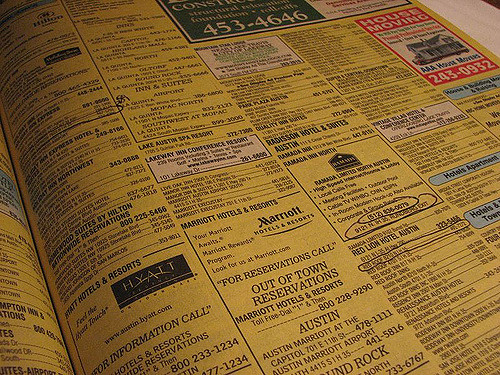
\includegraphics[width=0.9\textwidth]{images/phonebook.jpg}\\
		\hspace*{15pt}\hbox{\scriptsize Image By:\thinspace{\itshape mk ecker}}
		% https://www.flickr.com/photos/93678621@N00/247922018/
	\end{center}
		\column{0.455\textwidth}
		\begin{block}{I'm getting old}
			Who remembers these?
		\end{block}
			
	\end{columns}
\end{frame}

\begin{frame}
	\frametitle{Let's solve a problem!}
	\framesubtitle{Searching in a sorted list}
	
	\begin{columns}
		\column{0.505\textwidth}
	\begin{center}
		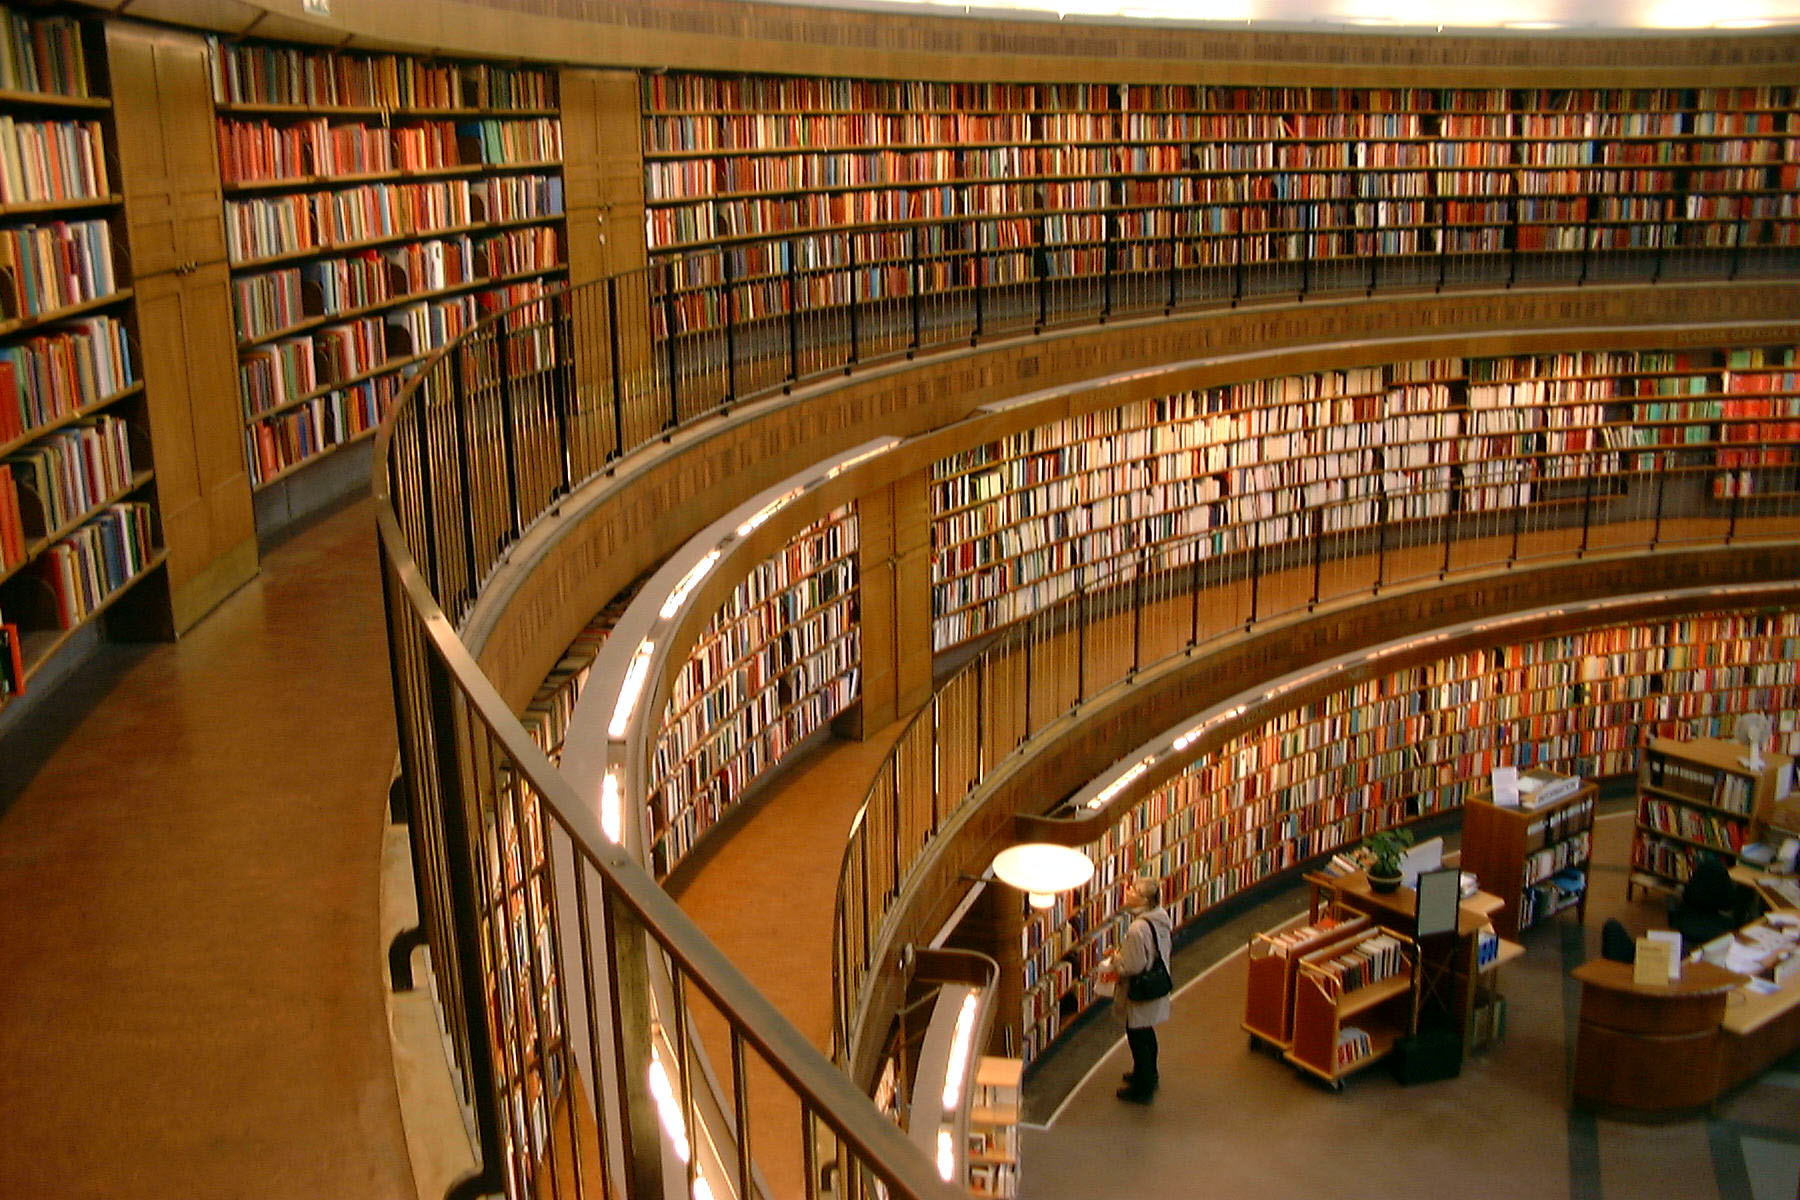
\includegraphics[width=0.9\textwidth]{images/library.jpg}\\
		\hspace*{15pt}\hbox{\scriptsize Image By:\thinspace{\itshape Marcus Hansson}}
		% https://commons.wikimedia.org/wiki/File:Interior_view_of_Stockholm_Public_Library.jpg
	\end{center}
		\column{0.455\textwidth}
		\begin{block}{Even for this}
			How do you look for books in a library? Say for instance you look for ``To kill a mockingbird'' by Harper Lee.
		\end{block}
		\pause
		\begin{block}{Well...}
			\begin{itemize}
				\item You see ``Split second'' by David Baldacci and you need to look further down the shelf.
					\pause
				\item You see ``The Amber Spyglass'' by Philip Pullman and you need to go back\dots
					\pause
				\item Let's formalise that idea!
			\end{itemize}
		\end{block}
	\end{columns}
\end{frame}

\begin{frame}
	\frametitle{Recursion}
	\framesubtitle{Recursion}
	\begin{center}
		
\includegraphics[width=0.8\textwidth]{images/google.png}\\
		\hspace*{15pt}\hbox{\scriptsize Source: Google}
	\end{center}	
\end{frame}

\begin{frame}
	\frametitle{Déjà Vu all over again?}
	
		\begin{block}{Recursion}
			A recursive function is a function that calls itself.
		\end{block}	
		\pause
		\begin{columns}
			\column{0.455\textwidth}
			\begin{block}{Fibonacci}
				For instance for Fibonacci:
				\begin{align*}
					F(1) &= 1 \\
					F(2) &= 1 \\
					F(n) &= F(n-1) + F(n-2) \text{ if $n > 2$}\\
				\end{align*}
			\end{block}
			\column{0.455\textwidth}
			\pause
		\lstinputlisting{src/fib.py}
				
		\end{columns}
\end{frame}

\section{Binary Search}
\label{sec:binary_search}


\begin{frame}
	\frametitle{Binary Search}
	\framesubtitle{Don't worry, there's no zeroes and ones involved}

	\begin{block}{Binary search}
		Given a sorted list $L$, determine if it contains an item with value $v$.
	\end{block}
	\pause
	\begin{block}{Example: Sorted names}
		\texttt{L = [Angelova, Chong, Hugtenburg, Sijm, van den Akker]}\\
		Does it contain \texttt{Sijm}?\\
		Answer: Yes!\\
		\pause
		\alert{But how do we get there?}
	\end{block}
	\pause
		\begin{block}{Sublinear time}
			Remember that \texttt{in} from Python takes $\Theta(n)$ time. We want to improve on that!
		\end{block}	
\end{frame}

\begin{frame}
	\frametitle{Binary search}
	\framesubtitle{The idea}
	
	\begin{overlayarea}{\textwidth}{\textheight}
		Let's build this algorithm:
		\pause
			\begin{columns}[t]
					
				\column{0.455\textwidth}
		\begin{enumerate}
			\scriptsize
			\only<6->{\item If the list is empty, return false}
		\item \only<6->{Otherwise\dots}Take the middle element of the list\only<7->{ with index \texttt{m}}, with value $x$.
		\item If $x = v$, return true.
		\pause
		\item If $x > v$, \alt<8->{return binary search in \texttt{L[:m]}.}{start looking in the \alt<5->{left}{\_\_\_} side of the list.} 
		\item If $x < v$, \alt<8->{return binary search in \texttt{L[m+1:]}.}{start looking in the \alt<5->{right}{\_\_\_} side of the list.}
		\end{enumerate}
				\column{0.605\textwidth}
		\only<11->{
			\lstinputlisting{src/binary-search.py}	
		}
			\end{columns}
		\only<4>{
			\begin{block}{Filling in the blanks}
				\small
				What should we put on the blanks?
				\vspace*{-10pt}
				% \begin{multicols}{2}
				\begin{enumerate}[A.]
					\item `left' on line 3 and `left' on line 4. 
					\item `left' on line 3 and `right' on line 4. 
					\item `right' on line 3 and `left' on line 4. 
					\item `right' on line 3 and `right' on line 4. 
					\item I don't know.
				\end{enumerate}	
			% \end{multicols}
			\end{block}
		}
		\only<9>{
			\begin{block}{Pseudocode}
				The above is what some might call \textit{pseudocode}. A natural language description of our program.			
			\end{block}	
		}
		\only<10>{
			\begin{block}{Let's do an example!}
				But just on the board, rather than in the slides.
			\end{block}	
		}
	\end{overlayarea}
\end{frame}

\begin{frame}
	\frametitle{So how well does this do?}

		\begin{block}{Reminder}
			Our time to beat is the Python built-in \texttt{in} operator that requires $\Theta(n)$ time!
		\end{block}	
		\begin{columns}
			\column{0.605\textwidth}
				\lstinputlisting{src/binary-search.py}	
			\column{0.405\textwidth}
			\pause
			\begin{block}{T(n)}
				What is the runtime of this function? 
				Try to formulate a recursive $T(n)$, where $n$ is \texttt{len(L)}.
			\end{block}	
			\pause
			\begin{block}{T(n)}
				$T(0) = c_0$ for lines 5 and 6.\\
				$T(n) = T(\lfloor n/2 \rfloor) + c_1 + c_2n$ for lines 8 through 15.
			\end{block}
		\end{columns}
\end{frame}

\begin{frame}
	\frametitle{So how well does this do? In terms of space}

		\begin{columns}
			\column{0.605\textwidth}
			\lstinputlisting{src/binary-search.py}	
			\column{0.405\textwidth}
			\begin{block}{S(n)}
				What is the runtime of this function? 
				Try to formulate a recursive $S(n)$, where $n$ is \texttt{len(L)}.
			\end{block}	
			\pause
			\begin{block}{S(n)}
				$S(0) = c_0$ for lines 5 and 6.\\
				$S(n) = S(\lfloor n/2 \rfloor) + c_1 + c_2n$ for lines 8 through 15.
			\end{block}
		\end{columns}
\end{frame}

\begin{frame}
	\frametitle{No improvements}
		\begin{block}{Reminder}
			Our time to beat is the Python built-in \texttt{in} operator that requires $\Theta(n)$ time!
		\end{block}	
		\begin{block}{Making it strictly better}
			This is still $O(n)$ at least... Because we make copies of the list in lines 13 and 14.	\\
			How about we two more parameters: lowest index, largest index instead of a copy of half of the list.\\
			Now we only have $T(n) = T(n/2) + c_1$.
		\end{block}	
\end{frame}

\begin{frame}
	\frametitle{How do we solve this?}

	\begin{block}{Recurrence Equations}
		How do we get to $O(...)$ now?
	\end{block}
	\pause
	\begin{block}{Repeated unfolding}
		$T(n) = T(n/2) +c_1$, so $T(n/2) = T(n/4) + c_1$.\\
		Substituting this, we get: $T(n) = T(n/4) + 2c_1$.
	\end{block}
	\pause
	\begin{block}{As a computer scientist...}
		To make the math a little `cleaner' we will assume $n = 2^m$ for some integer $m \geq 0$.	
	\end{block}
\end{frame}

\begin{frame}
	\frametitle{Solving it: getting a closed form}

	Repeated unfolding:
	\begin{align*}
		T(n) &= T(\lfloor n/2 \rfloor) + c_1\\
				 &= T(\lfloor n/4 \rfloor) + 2c_1\\
				 &= T(\lfloor n/8 \rfloor) + 3c_1\\
				 &= T(\lfloor n/2^k \rfloor) + kc_1\\
		\intertext{Take $k= \log_2(n+1)$ to get to $T(0)$}
		     &= T(\lfloor n/2^{\log_2(n+1)} \rfloor) + c_1\log_2(n+1)\\
				 &= T(0) + c_1\log_2(n+1)\\
				 &= c_0 + c_1\log_2(n+1)
	\end{align*}
\end{frame}

\begin{frame}
	\frametitle{Confirming our `repeated unfolding'}
	\begin{block}{How do we know it works?}
		How do we know this `guess' is correct?	
	\end{block}
	\begin{block}{Induction!}
		Induction! (Let's see what you think of my idea of induction ;))
	\end{block}
\end{frame}

\begin{frame}
	\frametitle{Proof by induction}
	\framesubtitle{For powers of 2}
	\begin{proof}
		To prove: $T(n) = c_0 + c_1 \log_2(n)$ for $T(n)= \begin{cases}
			c_0 & \text{ if n = 1}\\
			T(n/2) + c_1 & \text{ else}
		\end{cases}$.	\\
		Base case ($n=0$): $T(0) = c_0 = c_0 + c_1 \cdot 0 = c_0 + c_1\log_2(0+1)$.\\
		Inductive case:
		Assume for arbitrary $k$: $T(k) = c_0 + c_1 \log_2(k+1)$. (IH)\\
		\vspace*{-15pt}
		\begin{align*}
			T(2k) &= T(2k/2) + c_1\\
					 &= T(k) + c_1\\
					 &=_\text{\small IH} c_0 + c_1\log_2(k+1) + c_1\\
					 &= c_0 + c_1(\log_2(k+1) + \log_2(2))\\
					 &= c_0 + c_1(\log_2(2(k+1)))
		\end{align*}
		Since $k$ was arbitrarily chosen, it holds for all $n \geq 0$.
	\end{proof}
\end{frame}

\begin{frame}
	\frametitle{So...}
		\begin{block}{Main take-away}
			Searching in an unsorted list: $O(n)$.\\
			Searching in an sorted list: $O(\log(n))$.
		\end{block}	
		\pause
		\begin{block}{So\dots}
			Does that mean we should always sort our list?
		\end{block}
		\pause
		\begin{block}{It depends}
			It depends\dots\\
			We will find out when we discuss sorting in week 3!
		\end{block}
\end{frame}